\chapter{腹部肿块}

腹腔内的器官和组织由于各种原因而发生肿大、膨胀、增生、粘连或移位,致形成腹腔内异常的包块而被触及,称为腹部肿块。腹部肿块多数来自腹腔内疾病,少数来自腹膜后病变。其性质可归纳为肿瘤性、炎症性、梗阻性、潴留性、损伤性和先天性等,涉及内、外、妇、儿科疾病,是临床诊断难题之一。

\section{【腹部肿块与腹壁肿块、假性肿块的区别】}

腹部肿块须和腹壁病变所致的肿块相区别。腹壁肿物如脂肪瘤、腹壁脓肿、脐部囊肿等,位置较表浅,可随腹壁移动;当患者坐位或收紧腹肌时,肿物更显著,腹肌松弛时肿物即较不明显。

进一步则须判定该肿块是腹腔内真性肿块抑或假性肿块。正常腹部可触及的包块包括:腹直肌肌腹、横结肠、腰椎椎体、腹主动脉等。长期便秘者,粪块可积聚于乙状结肠甚至盲肠内,触诊时可在局部摸到相当硬实的包块,清洁灌肠或服泻药排除积粪后包块即消失;膀胱尿潴留时在耻骨上部也可触及圆形隆起的肿物,排尿或导尿后肿物即消失。成年女性腹部包块需注意子宫妊娠的可能性,此时有停经史及其他妊娠征象可助诊断。腹外疝如脐疝、腹股沟疝、股疝,其特征是时隐时现,增加腹压时包块增大,咳嗽时可触到膨胀性冲动感,如疝内容物是肠管,听诊可闻肠鸣音。须注意腹股沟疝包块经常可坠入阴囊,体检不要漏掉外生殖器检查。

\section{【腹部肿块的---般鉴别诊断】}

腹部肿块有下列的一些规律性和特点,有助于提示诊断:

\subsection{(一)年龄、性别与个人史}

婴幼儿多考虑先天性疾病或肠套叠,青少年多为肠结核、克罗恩病,女性患者注意妊娠和排除妇科疾病,牧区患者注意包虫病(棘球蚴病)。

\subsection{(二)腹部肿块形成的过程}

腹内肿块长时间存在,且生长缓慢而无明显症状者,大多属良性,如脂肪瘤、囊肿等。在腹部受撞击后短期内迅速出现的肿块常为内出血并有血肿形成。如肿块在腹部受伤后一段时间始出现者,应考虑胰腺或肠系膜囊肿的可能。如患者曾与狗有密切接触,则应考虑腹腔内包虫病(棘球蚴病)的可能。肿块如在高热、寒战、腹痛与白细胞增多等情况下发生者,提示腹腔内有脓肿形成。

\subsection{(三)腹部肿块的部位}

腹部肿块一般起源于所在部位的脏器(参见图\ref{fig25-1}及表\ref{tab29-1}),但肿块过小时不易触及,过大时则难以确定其起源部位。尤以腹腔内炎性包块、恶性肿瘤,往往范围广泛,部位不一,难以确定其起源的部位。有些发生解剖上变异,如游走肾、游走脾可离开原位出现;高位阑尾肿块也可移至肝下。肿块的定位诊断有时还需行有关的腹外检查,如上腹部肿块有时是由膈下脓肿或胸腹主动脉瘤引起的,这时需行胸部检查协助诊断。下腹部肿块有时是因睾丸未下降引起,这时应行外生殖器检查以明确诊断。

\begin{table}[htbp]
\centering
\caption{腹部肿块的部位与疾病分类}
\label{tab29-1}
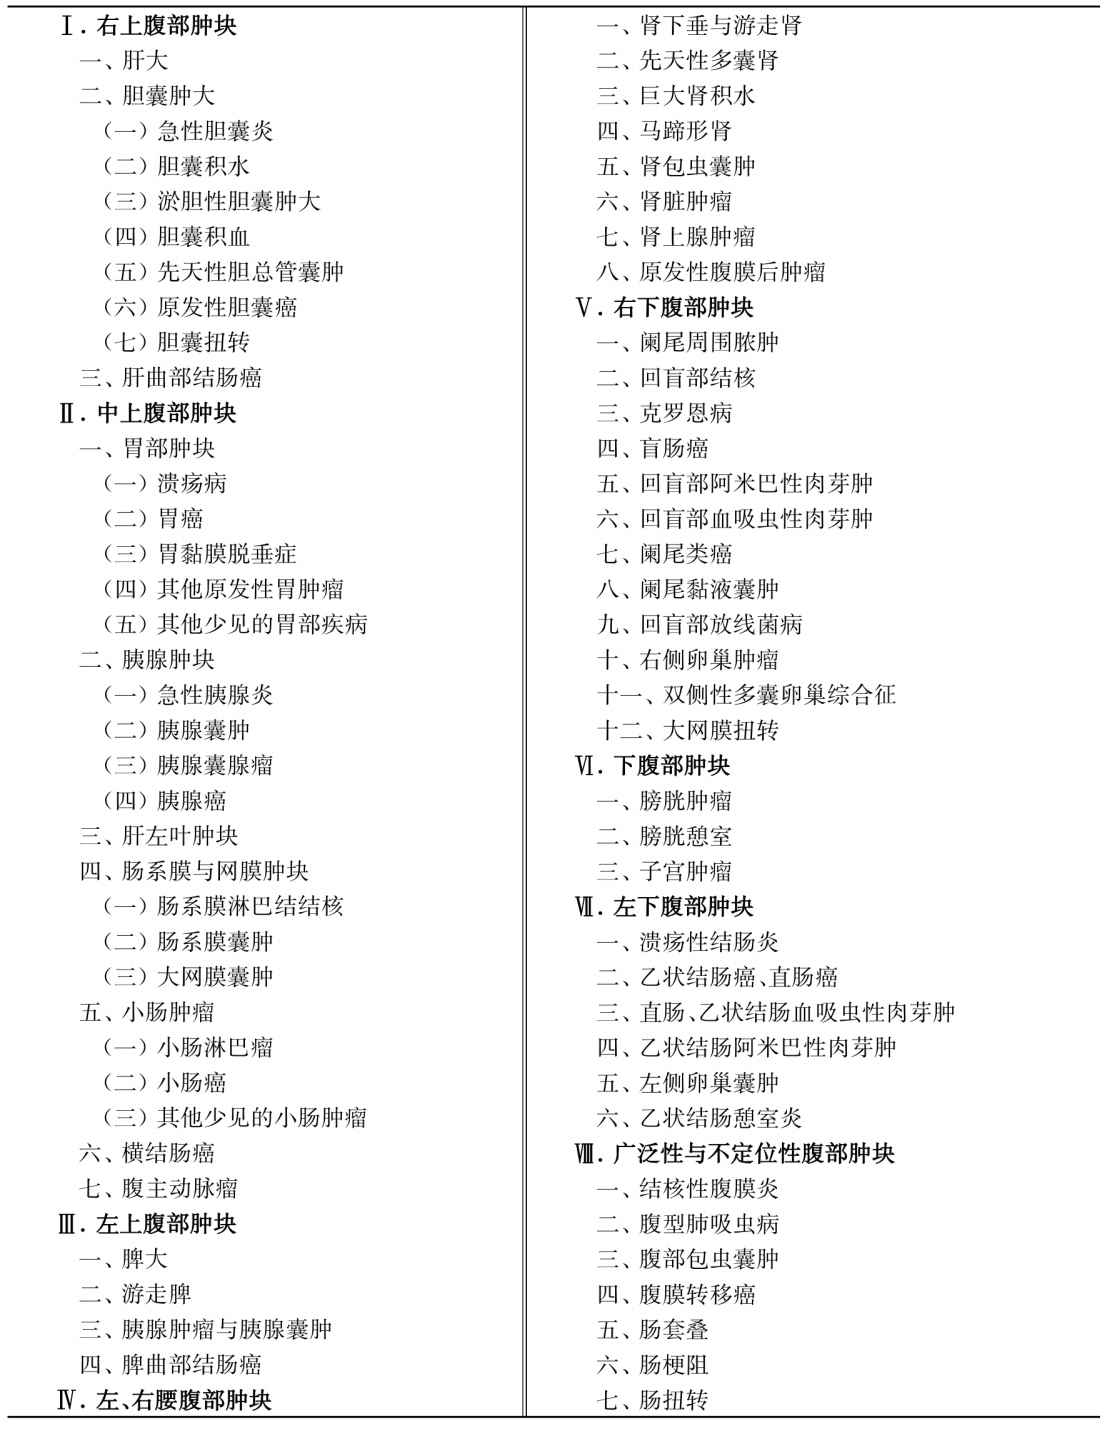
\includegraphics[width=5.91667in,height=7.61458in]{./images/Image00154.jpg}
\end{table}

\subsection{(四)腹部肿块的性状}

1.右上腹梨形肿块常为增大的胆囊。表面平滑、质硬而有弹性,下极(或两极)呈半圆形者提示为肾脏。呈香肠形者多见于肠套叠、肠梗阻等。如包块大小变化不定,甚至可消失,可能为充气的肠曲引起。通过腹部叩诊和听诊可以鉴别空腔脏器和实质脏器肿块。

2.肿块表面平滑呈囊样感者,可见于胰腺、胆总管、肠系膜、网膜以及卵巢等器官的囊性肿物,或腹部包虫病(棘球蚴病),或肾盂、胆囊的积水。

3.肿块外形不规则或表面呈结节状而质地坚硬者,常提示为腹腔内恶性肿瘤。

4.肿块上缘的境界清楚,而下缘模糊不清者,应多考虑为卵巢的肿瘤。

5.包块能用手推动者,可能来自胃、肠或肠系膜。肠系膜肿块可左右移动,但上下移动则受限,移动范围广、距离大的肿物多为带蒂肿物。肿块随体位改变而上下移动者,可能为内脏下垂。肿块在未与周围组织粘连或尚未蔓延至附近组织时,可随呼吸上下移动者,多起源于胃、横结肠、肝、脾、肾等(肝、脾随呼吸移动性较显著);起源于胰、腹膜后、下腹部脏器的肿块及腹主动脉瘤,一般不随呼吸移动。

6.肿块随大量排尿后迅速缩小,尿量减少时则增大,多为巨大肾积水。

7.肿块有膨胀性搏动者,常见于腹主动脉瘤与三尖瓣关闭不全所致的肝搏动。

8.有明显压痛的肿块多为炎性肿块,如结核性腹膜炎、阑尾周围脓肿、肝脓肿等。绞窄性肠梗阻出现的包块也有压痛。

\subsection{(五)腹部肿块与伴随症状及体征}

1.腹部肿块伴有腹痛、呕吐、腹胀、腹泻或便秘症状,多见于肠梗阻、慢性肠道肉芽肿、胃肠恶性肿瘤、克罗恩病等。

2.腹部肿块伴有黄疸,提示为肝、胆道与胰腺疾病或其他病变压迫胆道出口。伴恶病质者肿块常为恶性。脾大伴有黄疸可能为溶血性贫血。

3.腹部肿块伴有腹水,多见于结核性腹膜炎、原发性或继发性肝癌、腹膜转移癌、卵巢肿瘤等。

4.腹部肿块伴柏油样便可见于胃或小肠肿瘤;伴有血便应注意结直肠肿瘤、肠结核、克罗恩病以及肠套叠等。

5.腹部肿块伴有膀胱刺激征、血尿、脓尿或尿潴留者,多为泌尿系统疾病,如膀胱肿瘤、多囊肾、肾肿瘤、肾积水(积脓)等。

6.腹部肿块伴有闭经或阴道出血者,应注意卵巢与子宫肿瘤、妊娠等。

7.腹部肿块伴有阵发性高血压、多汗,应考虑嗜铬细胞瘤。

8.腹部肿块伴有锁骨上淋巴结、腹股沟淋巴结肿大,应行淋巴结活检。肛门指检及妇科检查也可为诊断提供线索。

9.腹部肿块伴有寒战、高热、腹痛、血白细胞增高,多为炎性包块。

\section{【腹部肿块的实验室检查与器械检查】}

\subsection{(一)血液检查}

1.白细胞计数升高、中性粒细胞核左移者提示感染性疾病;嗜酸性粒细胞增多提示过敏及寄生虫疾病;严重贫血多见于恶性疾病;全血细胞减少可见于脾功能亢进、黑热病。

2.肝功能检查有助于肝胆疾病的诊断。

3.血中儿茶酚胺测定有助于嗜铬细胞瘤诊断。

4.卵巢绒毛膜癌者可有β-绒毛膜促性腺激素(β-HCG)升高。

5.血中肿瘤标志物如AFP、CEA、CA19-9、CA50、CA72-4、CA125、CA242等检查,有助于消化道肿瘤的诊断,联合检测意义更大。前列腺特异抗原(PSA)在前列腺癌时明显升高。

6.血清乳酸脱氢酶(升高)有助于良恶性肿块鉴别。

\subsection{(二)尿液检查}

尿常规有助于泌尿系统肿块的诊断,24小时尿中3-甲氧基-4-羟苦杏仁酸(VMA)及尿儿茶酚胺的测定有助于嗜铬细胞瘤诊断。

\subsection{(三)粪便检查}

大便常规检查可了解有无寄生虫疾病;长期大便隐血阳性应考虑胃肠道及胆道肿瘤的可能。

\subsection{(四)超声波检查}

B超可诊断腹腔实质性脏器的占位性病变,对病变大小、范围、周围淋巴结以及与邻近器官关系可作出判断,并可判断肿块的良恶性。还可以在超声引导下穿刺活检进行病理组织学检查。近年腔内超声因更接近检查脏器,受肠气等影响小,因而准确性更高,如经直肠前列腺超声检查和经阴道妇科B超检查。还可根据需要进行术中超声检查。

\subsection{(五)X线检查}

1.腹部平片可明确是否存在肠梗阻;有无膈肌抬高、运动受限及是否合并腹水;以及有无钙化、牙齿、骨阴影,以帮助确定是否为畸胎瘤。

2.X线钡剂造影检查钡餐可观察胃、小肠有无狭窄、充盈缺损、憩室、受压表现、蠕动情况及扭转征象,钡剂灌肠也可同样了解大肠上述情况。

3.胆道造影经皮经肝穿刺胆管造影(PTC)、内镜下逆行胰胆管造影(ERCP)对胰胆管、胆囊及壶腹部病变有较高的诊断价值。

4.肾盂造影及腹膜后充气造影有助于泌尿系统及腹膜后疾病的诊断。

\subsection{(六)内镜检查}

胃镜、十二指肠镜、(单)双气囊小肠镜、结肠镜可以直接观察胃肠黏膜病变,膀胱镜也可直接观察病变,并可取活检行病理检查,常可帮助明确诊断。无创伤性胶囊内镜检查主要观察小肠黏膜,可帮助诊断小肠疾病,缺点是不能调控方向及行病理学检查。胶囊结肠镜可帮助筛查结肠肿瘤和息肉以及观察结肠IBD情况,尤其是溃疡性结肠炎的诊断和病情评估。腹腔镜检查对腹部肿块诊断有重要意义,可直接观察腹腔内及腹膜病变,并取活检明确诊断,对某些疾病还可同时进行治疗。超声胃镜、超声肠镜有助于黏膜下肿瘤、外压性病变、肿瘤浸润深度以及周围淋巴结肿大的诊断,对诊断胃、肠、胰、胆道肿瘤及肿瘤术前分期有较大意义,对个别腹部超声、腹部CT未能诊断的胆总管及胰腺病变,选择超声胃镜检查可帮助诊断。CT仿真内镜通过三维模拟成像可帮助无创诊断胃肠病变。

\subsection{(七)CT检查}

CT对腹部实质性脏器病变及腹腔、空腔脏器占位病变诊断具有重要价值,可清晰显示病灶大小、与邻近器官关系、有无淋巴结肿大,帮助诊断炎症性、损伤性、先天性及肿瘤性病变。目前在急腹症的诊断与鉴别诊断中,被认识到正发生日益重要的作用。CT小肠造影(CTE)对小肠克罗恩病(CD)的诊断意义较大。可观察肠壁、肠系膜、淋巴结及腔外并发症如瘘、脓肿、窦道等,是诊断和随访CD的重要检查。具有扫描速度快、图像质量高、费用相对较低等特点。

\subsection{(八)MRI检查}

主要用于肝内占位性病变的鉴别诊断,通过磁共振胰胆管造影(MRCP)可帮助诊断胰胆病变。近年磁共振小肠造影术(magnetic
resonance
enterography,MRE)的应用日益增多,它无辐射,也可观察肠壁及肠外病变,缺点是扫描速度慢,费用比CT高。

\subsection{(九)放射性核素检查}

可用于梅克尔憩室异位胃黏膜显像以及肝胆道显像,由于特异性较差,目前较少选用。

\subsection{(十)选择性腹腔动脉造影}

对动脉瘤、肝脏占位病变及腹腔内脏器官肿瘤具有很好的诊断价值。

\section{【腹部肿块的病因分类】}

腹部肿块的病因很多,为了叙述方便,按腹块的部位及其常见的疾病(见表\ref{tab29-1})顺序讨论于下。

\protect\hypertarget{text00229.html}{}{}

\section{98 右上腹部肿块}

\subsection{98.1 肝大}

参见第30章。

\subsection{98.2 胆囊肿大}

\subsubsection{一、急性胆囊炎}

急性胆囊炎时胆囊往往肿大,但常因腹壁紧张而难于触及,少数病例可在右肋缘下能触及梨形肿大的胆囊(参见第78.1节)。

\subsubsection{二、胆囊积水(化学性胆囊炎)}

胆囊积水是由于胆囊管阻塞,胆汁滞留于胆囊内,胆色素渐被吸收并引起化学性刺激,而发生轻度慢性胆囊炎,同时胆囊黏膜不断分泌黏液,使胆囊逐渐扩大。腹部检查在胆囊区可触及表面平滑而有囊样感的梨形肿块,有轻度压痛或无压痛,临床症状类似慢性胆囊炎。超声检查可协助诊断。此病的确诊主要依靠手术检查,其治疗方法是摘除积水的胆囊。

\subsubsection{三、淤胆性胆囊肿大}

由于肝外胆道梗阻所致的无痛性淤胆性胆囊肿大,可见于壶腹癌及胰头癌,B超、CT检查有一定的鉴别诊断意义,必要时可行ERCP或PTC检查。

\subsubsection{四、胆道蛔虫症}

蛔虫钻入胆道可引起疼痛,当合并胆道感染时,可出现畏寒、发热和黄疸,感染严重时,胆囊可触及肿大并有压痛。超声检查、胃镜及ERCP可帮助诊断。

\subsubsection{五、先天性胆总管囊肿}

先天性胆总管囊肿(先天性胆总管囊性扩张症)是并不十分少见的先天性疾病。患者大多数是女性青少年与儿童。在右上腹可触及表面平滑、富有弹性和轻度压痛的椭圆形肿块。此病的临床诊断主要根据是:①腹痛、黄疸和腹块为本病的典型症状,但很少同时发生;②右上腹肿块比较固定,不随呼吸移动,肿块与肝脏分隔,可在数天内迅速增大;③腹痛多为不经常的钝痛,偶呈绞痛,多无放射痛,疼痛发作时常伴有恶心、呕吐;④间歇性发热;⑤间歇性出现阻塞性黄疸。B超与X线检查对诊断有很大意义,特别是囊肿不太大,临床上不易触及时,必要时可行腹部CT检查。腹部平片可见右上腹致密肿块阴影。钡餐检查可见十二指肠受压向左下移位,结肠肝曲较正常位置为低。

此病一般根据以上临床特点与B超或X线、CT检查,术前多可获得正确诊断,必要时可行PTC或ERCP检查,但少数病例须经手术探查方能最后确诊。

此病在临床上需注意与肝包虫囊肿、胰腺囊肿、肠系膜囊肿相鉴别(参见本章有关内容)。

\subsubsection{六、原发性胆囊癌}

原发性胆囊癌临床少见,多发生于50岁以上的女性。癌肿的类型以弥漫型腺癌为多。最常见而较早期的症状是右上腹痛。其他主要症状是阻塞性黄疸、食欲不振、体重明显减轻与上腹部肿块。胆囊癌转移较迅速,癌细胞可直接浸润邻近器官,如肝、十二指肠、胃、结肠与腹膜。当肿瘤发生胆囊外浸润时可与邻近组织粘连成块。较晚期病例,在右上腹可触及无明显触痛、较固定而质坚实的肿块。B超与CT有助于诊断。必要时可行剖腹探查以确诊。

\subsubsection{七、胆囊扭转}

胆囊完全扭转发病急剧,突发右上腹剧烈持续性绞痛,放射至肩胛背部,常伴有恶心呕吐。在右上腹出现有明显压痛,可随呼吸移动的肿块(参见第78.3节)。

\subsection{98.3 肝曲部结肠癌}

肝曲部结肠癌可形成右上腹部坚实的结节性条状肿块而被触及(参见第80.3节)。

\protect\hypertarget{text00230.html}{}{}

\section{99 中上腹部肿块}

\subsection{99.1 胃部肿块}

\subsubsection{一、消化性溃疡}

单纯的胃十二指肠溃疡不产生上腹部包块。慢性穿透性溃疡与周围组织粘连,有时可在上腹部形成边缘不清、有压痛的包块。患者腹痛较剧烈,无节律性,疼痛常向背部放射,药物疗效不佳。常伴有食欲不振、体重减轻、贫血、消瘦。大便潜血可持续阳性。临床上易与胃恶性肿瘤混淆,内镜与X线胃肠钡餐检查可助诊断。

幽门梗阻常伴有胃部振水音,可见胃逆蠕动波。溃疡病并发器质性幽门梗阻时,通过病史问诊、体格检查与内镜检查可作出诊断。

\subsubsection{二、胃 癌}

胃癌患者在能触及腹部肿块时一般已属中晚期。肿块位于中上腹者最多,右上腹者次之,左上腹者最少。

胃癌的肿块较为坚实,境界不清,外形不规则,多无明显压痛,多数可以推动,早期可随呼吸移动,但晚期则固定。如癌已直接浸润或转移至邻近器官(如淋巴结、大网膜),则可形成较大的团块。晚期胃癌的典型征象是:腹部肿块、恶病质和呕吐,呕吐物往往呈咖啡渣样。此时常已有淋巴结转移,尤其左锁骨上淋巴结转移。X线钡餐、CT和胃镜检查对胃癌有重要诊断价值(参见第81.2节)。

\subsubsection{三、胃黏膜脱垂症}

较重的胃黏膜脱垂症,有时可在幽门区触及一软性肿块,如核桃大(参见第81.2节)。

\subsubsection{四、胃间质瘤}

胃肠道间质瘤(gastrointestinal stromal
tumor,GIST)是消化道最常见的间叶源性肿瘤,胃最多见,其次见于小肠;胃肠道外间质瘤较少见,主要见于肠系膜、腹膜、腹膜后。患者最常见消化道出血,包括呕血、便血或大便隐血,通常由黏膜溃疡引起,其他症状包括上腹不适、腹痛、腹部肿块等。

\subsubsection{五、其他原发性胃肿瘤}

良性胃肿瘤(如腺瘤)体积较小,一般难以触及。

恶性胃肿瘤除胃癌之外,还有各类型胃肉瘤与胃霍奇金淋巴瘤。

\paragraph{(一)胃肉瘤}

胃肉瘤是比较罕见的胃恶性肿瘤,其中以淋巴肉瘤较为多见。国内报告有胃淋巴肉瘤、胃平滑肌肉瘤等。患者多为青壮年。胃肉瘤多生长于胃小弯与胃后壁,生长在幽门部者较少。肿瘤体积大,易出血,无明显消化障碍症状,长时间内不引起狭窄或向邻近器官转移与腹水。腹块并非早期常见的症状。患者常因上消化道急性出血或腹痛而就诊,症状与胃癌相似,但患者年龄大多较轻,病程较长,全身情况一般较好,与胃癌不同。X线检查可发现圆形、表面平滑与界限明显的充盈缺损。此瘤需经内镜或手术探查活检方能确定诊断。

胃平滑肌肉瘤有溃疡形成与继发感染时,可引起局部淋巴结肿大,在剖腹探查时难与胃癌区别,或认为是已发生广泛蔓延的胃癌而放弃手术。如肿瘤位于胃体部,须考虑平滑肌肉瘤的可能性。此瘤转移较晚,恶性度低。即时作冰冻切片有助于鉴别;如为平滑肌肉瘤,可使患者获得手术根治的机会。

\paragraph{(二)胃霍奇金淋巴瘤}

胃霍奇金淋巴瘤是比较少见的胃部疾病,多发生于青壮年男性。常见的症状是上腹痛、恶心、呕吐、消化不良、消瘦、黑便、呕血、贫血,晚期左上腹部可触及肿块。此病在X线检查时也常难与其他胃部肿瘤鉴别,往往需经胃镜病理活检与手术探查方能确诊。

\subsubsection{六、其他少见的胃部疾病}

\paragraph{(一)胃扭转}

胃扭转有时可在上腹部触到拳头大肿块,其边缘不清,质软,有振水音。症状缓解时此肿块也消失。患者的主要症状为发作性上腹部胀痛、呕吐,也可有呕血与便血。胃扭转多为慢性型,X线检查和胃镜有助于明确诊断(参见第81.2节)。

\paragraph{(二)胃放线菌病}

胃放线菌病临床上非常罕见,其主要临床表现是上腹部肿块,轻度胀痛,伴有食后不适、嗳气、反酸、上腹闷胀、体重明显减轻。肿块质韧,表面平滑,境界不清,可移动,无明显压痛。此病往往需经内镜或手术探查病理活检方能确诊。

\paragraph{(三)胃石症}

胃石症由毛发、植物纤维果实构成,在我国以柿子为多见。柿子在胃酸作用下形成团块,不能通过幽门而滞留于胃,不断堆积增大。患者可有上腹闷胀不适或疼痛,伴有恶心呕吐,上腹可触及一包块,质较硬,可自由推动无压痛,患者有进食上述异物病史可提示本病诊断,胃镜检查可以确诊。

\subsection{99.2 胰腺肿块}

\subsubsection{一、急性胰腺炎}

少数重型急性胰腺炎患者,有时在上腹部或脐部可触及边缘不清、有压痛的肿块,可能由于局限性腹膜炎、胰腺脓肿或囊肿形成所致。

\subsubsection{二、胰腺囊肿}

胰腺囊肿可分为真性和假性两大类,前者临床上少见,囊肿体积较小,无特殊临床表现;后者临床上较多见,约2/3病例继发于急性或慢性胰腺炎,其余是由于胰腺创伤及其他原因所致。假性囊肿患者多有急性胰腺炎或腹部外伤史。囊肿发展迅速,数天或数星期内即可被触及,多位于上腹偏左(因多发生于胰腺体部或尾部),肿块大小不一,呈球形或椭圆形,表面平滑,有囊样感,压痛不明显,一般不易推动,此点可与肠系膜或网膜囊肿区别。大的胰腺囊肿可向下伸延至盆腔,因此在女性患者应与卵巢囊肿鉴别;卵巢囊肿是自下向上伸展,此病则相反,且早期即出现消化不良症状。若囊肿向上发展达胃、肝之间,需与肝肿瘤、肝包虫囊肿或巨大胆囊积水相区别。此病与肾囊肿或其他腹膜后囊肿,在位置上不易鉴别,须靠X线及泌尿系检查。在临床上凡有下列情况者应考虑到胰腺假性囊肿的可能性:①急性胰腺炎或胰腺创伤后,上腹部出现囊性肿块,并逐渐增大;②伴有上腹痛或不适感,食后腹胀闷、恶心、呕吐、食欲不振等消化功能紊乱;③超声检查提示为囊性肿块。X线检查对此病的诊断有重要意义。胃肠钡餐透视及腹平片可发现上腹部有密度增高的圆形或椭圆形阴影,有的可见囊壁钙化,胃、十二指肠、结肠因受压而移位与变形。B超和CT检查可确诊此病。

\subsubsection{三、胰腺囊腺瘤}

此病临床上少见,多发生于中年女性。腹部肿块往往是唯一的体征,临床上与胰腺囊肿难以区别,但其质较硬,患者并无急性胰腺炎史。早期可无症状。后期当肿块增大时可出现腹痛、疲乏、无力、体重减轻等症状。此病生长缓慢,多位于胰腺的体尾部或尾部。如肿块位于左上腹、近脐处有凹陷时触及,可误诊为脾大。B超与X线钡餐和CT检查可协助诊断。

\subsubsection{四、胰腺癌}

胰腺癌与壶腹周围癌能触及肿块时已属晚期。腹部肿块在上腹部偏左或偏右,外形多不规则,呈结节状,质较硬,大都固定,少数可随呼吸稍有移动,可有轻度压痛(参见第81.3节)。近年,胃肠胰神经内分泌肿瘤发病有增多趋势,多学科联合有助于早期诊断。

\subsubsection{五、自身免疫性胰腺炎}

自身免疫性胰腺炎(autoimmune
pancreatitis,AIP)是一种以梗阻性黄疸、腹痛不适等为主要表现的特殊类型的胰腺炎,AIP的临床特征与胰腺癌有相似之处,常表现为胰腺肿块或肿胀,仅以临床表现不能明确鉴别两者。AIP可伴有胰腺外器官受累,如硬化性胆管炎、硬化性涎腺炎、类干燥综合征、肺门淋巴结肿大、间质性肺炎、间质性肾炎及腹膜后纤维化等。影像学:胰腺弥漫性或局灶性增大,有时伴有包块、边缘呈低密度;胰胆管弥漫性、局灶性狭窄。血清学:血清IgG或IgG\textsubscript{4}
升高,其他自身抗体阳性。组织学:胰腺活检示淋巴浆细胞浸润伴纤维化,有大量IgG\textsubscript{4}
阳性细胞浸润。类固醇药物治疗可显著改善胰腺及胰腺外症状。对AIP及时正确的诊断可以指导其合理的治疗方案,避免不必要的手术。

\subsubsection{六、胰腺实性假乳头状瘤}

胰腺实性假乳头状瘤(solid pseudopapillary tumor of
pancreas,SPTP)是一种少见的低度恶性肿瘤,占胰腺肿瘤1\%~3\%,国内报告1180例荟萃分析,女性多见,男∶女为1∶8.37。发病年龄9~83岁,平均29岁。主要表现腹痛、腹胀(44.9\%),无明显症状体征,体检发现者(39.6\%),发现腹部肿块就诊者(11.2\%)。手术切除是首选治疗方法。肿瘤部位,胰体尾部(53.1\%),胰头(36.8\%),胰颈(8.7\%),偶发于胰腺旁、肠系膜、腹膜后。总体预后较好,5年生存率为95\%。

\subsection{99.3 肝左叶肿块}

肝左叶肿块可由于左叶肝癌、左叶阿米巴肝脓肿、左叶肝囊肿等所致。肝左叶肿块有时难与巨大胰腺囊肿相区别,但后者在胃肠钡餐X线检查时位于胃的后面,CT检查可明确诊断。

\subsection{99.4 肠系膜与网膜肿块}

\subsubsection{一、肠系膜淋巴结结核}

肠系膜淋巴结结核常为腹腔结核的一部分,单独存在者甚少。多见于儿童与青少年。肿大的肠系膜淋巴结常互相粘连成较大的团块,多在脐周或右下腹被触及,边界不明显,位置较深,质呈中等硬度,一般压痛不显著,移动性甚小。急性期常伴有右下腹或脐周剧痛、高热。慢性病例腹部X线平片可见钙化现象。可疑病例应作抗结核诊断性治疗,如疗效不佳时,宜考虑腹腔镜检查或手术探查以明确诊断(参见第81.6节)。

\subsubsection{二、肠系膜囊肿}

肠系膜囊肿是罕见的疾病,绝大多数发生于小肠系膜,多为淋巴管囊肿。可发生于任何年龄,小儿多见。淋巴管囊肿是一种先天性良性错构瘤,主要见于颈部、腋下,发生于小肠系膜很少见。大多无自觉症状或仅有腹部下坠感,体检则可发现脐部或右下腹肿块。囊肿显著增大压迫肠腔时,则出现腹痛与肠梗阻征象。肿块大多位于脐部右侧,表面平滑或稍隆凸,质较软,有囊样感与波动感,可向左右移动,但向上下活动度较小,也不随呼吸移动,如囊肿与周围组织粘连,或囊肿体积过大时,则无活动性。胃肠钡餐检查可发现肠外占位性变,由外伤、炎症、感染、腹部手术等因素导致局部淋巴管粘连、阻塞扩张、淋巴液淤滞,形成的囊肿属假性肠系膜囊肿。临床上须注意与胰腺囊肿、卵巢囊肿、腹膜后肿瘤、胃肠道肿瘤等鉴别。超声、CT检查提示为囊性肿块,细针抽吸穿刺活检可提高诊断率。此病往往需经手术探查方能确诊。

\subsubsection{三、大网膜囊肿}

大网膜囊肿临床上也属罕见,女性罹患多于男性。囊肿可为单房性或多房性,囊液可为浆液性、血性或乳糜性。其主要临床表现是腹部包块、腹痛或下坠感、贫血、消瘦、腹泻。肿块性质与肠系膜囊肿相似。巨大的囊肿往往易与腹水相混淆,但此病时胁腹部叩诊呈鼓音,并可听到肠鸣音,与腹水不同。X线检查对诊断有一定的帮助,钡餐透视与肾盂造影可排除消化道与泌尿系肿瘤。超声、CT检查提示囊性肿块。确诊往往须靠手术探查及病理学检查。

\subsection{99.5 小肠肿瘤}

原发于小肠的肿瘤,无论良性或恶性,均较其他部位为少。约2/3以上为恶性肿瘤,发病率男多于女,肉瘤发病年龄较癌平均约小10岁。

小肠良性肿瘤以腺瘤、间质瘤为最多见,多无症状,仅于出血、发生肠梗阻等并发症或其他腹部手术时始被发现。

小肠恶性肿瘤以腺癌及恶性淋巴瘤为多。患者有以下情况之一项或多项时,应注意小肠恶性肿瘤的可能:①最近体重明显减轻,食欲不振,经常有腹痛或未明原因的柏油样大便;②慢性腹泻、发热伴急性或慢性肠梗阻;③腹部肿块;④X线钡餐上消化道及钡剂灌肠检查或胃、肠镜检查胃及结肠均正常。

\subsubsection{一、小肠原发性淋巴瘤}

此瘤多发生于中年男性。病变部位以回肠较多见,其次为空肠;病理分类以网状细胞肉瘤、淋巴肉瘤最多,其次为霍奇金淋巴瘤;其主要症状是腹痛、局部压痛与肿块,腹部检查约50\%病例可触及肿块,多见于脐周。X线检查、内镜(小肠镜、结肠镜)检查对此病的诊断很有价值。必要时可剖腹探查,尤其是发现小肠扩张性病变及肠梗阻征象时有重要诊断意义。

\subsubsection{二、小肠癌}

小肠癌少见,多为腺癌,早期以腹部不适、腹痛、食欲减退、消瘦、贫血及腹泻等症状较为常见,晚期则可出现肿块、肠梗阻或(及)肠道出血等征象。诊断主要根据小肠X线检查,CT小肠造影。近年胶囊内镜及双气囊小肠镜的应用大大提高了本病的术前诊断率。

\subsubsection{三、其他少见的小肠肿瘤}

小肠良性肿瘤有腺瘤、平滑肌瘤、血管瘤、纤维瘤等,其中以腺瘤较为多见。小的肿瘤常无症状。如肿瘤向肠腔内增长,引起肠狭窄、肠套叠或肠扭转等并发症,则表现为急性肠梗阻的征象。在平时比较健康的情况下,出现急性肠梗阻而未发现任何原因,须注意小肠肿瘤的可能性。小肠平滑肌肉瘤是低度恶性的肿瘤,如向邻近组织或器官浸润、粘连,形成肿块时也可触及。

\subsection{99.6 横结肠癌}

主要表现便血、贫血、排便改变及肠梗阻表现,部分患者可在中上腹触及较硬肿块。

\subsection{99.7 腹主动脉瘤}

腹主动脉瘤少见,肿块多位于上腹部,可在腹部脊柱前被触及。肿块有膨胀性搏动,不随呼吸移动,多有压痛,消瘦的患者可触到震颤与听到滚筒样杂音。患者常有不同程度的腹痛。此病的诊断根据是:①有动脉硬化、梅毒或外伤的病史与上述的体征;②梅毒所致的腹主动脉瘤,梅毒血清反应常呈阳性;③X线平片可发现动脉瘤钙化斑、脊椎体受侵蚀现象,而椎间盘正常。多普勒超声与CT显示增宽的腹主动脉,可确定诊断。必要时可作腹主动脉造影以协助诊断。

\protect\hypertarget{text00231.html}{}{}

\section{100 左上腹部肿块}

\subsection{一、脾大(参见第31章)}

\subsection{二、游走脾}

脾脏离开其解剖位置而游动于腹腔其他部位时,称为游走脾。产生游走脾的原因颇多,主要是脾大及脾蒂与韧带的松弛,此外腹壁松弛和外伤也是诱因之一。游走脾临床上极少见,多发生于中年妇女,尤其是多次妊娠的经产妇或内脏下垂的患者。

游走脾的临床症状随其附近器官受牵引与压迫情况而异。胃被牵引时可出现腹痛、恶心、呕吐、嗳气;肠道受压可产生便秘;压迫子宫可使子宫移位;膀胱受压则有排尿困难;压迫直肠则有里急后重症状。

游走脾的诊断主要根据触诊与叩诊。正常脾脏所在部位的浊音区消失,而在腹腔其他部位出现无痛性、表面平滑、能活动且有弹性感而有切迹的肿块。超声波检查提示腹腔内实质性肿块,而脾区并无脾脏进出波,提示此处无实质性器官。如脾脏甚为活动,则臀高头低体位时能回复到左上腹。游走脾有时与左侧的肾脏不易区别,其不同点是:左肾的位置较为垂直且接近正中线,容易向上滑动,叩诊时其上有鼓音,边缘较为圆钝,无切迹可触及。游走脾发生扭转时,常易误诊为卵巢囊肿扭转或其他急腹症,往往须经手术探查方能明确诊断。

\subsection{三、胰腺肿瘤与胰腺囊肿(参见第99.2节)}

\subsection{四、脾曲部结肠癌}

脾曲部结肠癌有时可因癌组织增生并向周围组织浸润,致形成左上腹部坚实的肿块而被触及,但一般以肠梗阻、排便紊乱、便血等为主要表现,参见第82.2节。

\protect\hypertarget{text00232.html}{}{}

\section{101 左、右腰腹部肿块}

\subsection{一、肾下垂与游走肾}

正常肾脏在腹腔内一般不能触到,身体瘦弱的人则可触及位置较低的肾脏下极,钝圆形,质实而有弹性,表面平滑,当被触及时被检查者可出现恶心与不快感。肾脏移位可分为三级:第1级,仅能触及肾脏下极或肾体的一半;第2级,能触及整个肾脏;第3级,肾脏容易越过脊柱游动至对侧腹腔内(游走肾)。先天性异位肾与肾移位不同,前者肾脏不能被推回肾窝内。

超声检查与静脉肾盂造影检查有助于肾下垂的诊断。正常人仰卧位与直立位肾造影,肾脏上下活动度的差异为20~50mm,超过50mm时则诊断为肾下垂。

肾下垂与游走肾多发生于20~40岁之间的瘦长体型的女性。多见于右侧,但也可为两侧性。临床上多无症状,如有症状,一般为腰酸、腰痛、血尿、消化不良、厌食、嗳气、神经衰弱症状等。

\subsection{二、先天性多囊肾}

先天性多囊肾分婴儿型与成人型,前者病情严重,多于1岁内死亡,后者病变较轻,起病缓慢,多于成人以后才发病,此病大多数是双侧性,但往往一侧比较明显。一侧性者以左侧较常见。多囊肾可以很大,常较正常肾增大5~6倍,形状近似球形,表面呈结节状,质较韧,波动感多不明显。其临床表现随肾功能损害的程度而异。最早期囊肿较小,患者无症状或仅有腰部不适或钝痛,随囊肿的增大,腰痛因体力劳动而加剧,从一侧发作性腰痛转为双侧持续性;中期则出现头痛、呕吐、高血压、血尿、管型尿与蛋白尿等症状,晚期则出现尿毒症症状。

临床上若患者有下列表现之一时,应考虑先天性多囊肾的可能:①双侧肾区触及肿块,特别是呈结节状者;②单侧肾脏肿大,尿比重低而固定者;③肾区肿块并有血尿或(及)高血压表现者。

先天性多囊肾须与单纯性肾囊肿及肾包虫囊肿相鉴别。后两者无类似肾炎的病征与高血压。肾包虫囊肿患者体内常同时有其他器官的包虫病(棘球蚴病),血中嗜酸性粒细胞增多,包虫抗原皮内试验阳性。巨大多囊肾与卵巢囊肿的区别,可行双合触诊检查,后者囊肿起源于盆腔,肿块是自下向上生长。此外,本病也常需与肾肿瘤及肾积水鉴别,多囊肾为双侧性,肿大肾脏表面呈凹凸不平的囊肿而稍能移动,与晚期肾肿瘤坚实而固定不同。多囊肾波动感多不明显,有别于肾积水。超声(或CT)检查及肾盂造影对本病的诊断有重要价值。

\subsection{三、巨大肾积水}

一般以内容1000ml以上的肾积水称为巨大肾积水,可由于先天性肾盂、输尿管连接部狭窄、肿瘤或结石等阻塞所致。此病临床上少见,主要症状是腹部囊性肿块,此外可伴有腹痛、腰痛、血尿等症状。如为间歇性巨大肾积水,则大量排尿后肿块骤然缩小,或尿量减少时肿块迅速增大。此病的诊断根据是:①腹部有一侧性逐渐胀大的囊性肿块;②肿块向后伸延至骶棘肌外缘,有波动感;③尿液检查一般无明显异常;④超声检查提示为腰腹部充满液体的囊性肿块;⑤静脉肾盂造影患侧不显影,而健侧显影正常,逆行肾盂造影显示患侧输尿管向对侧移位及输尿管上端有梗阻。疑难病例经上述检查仍未能确诊时,可试行B超定位经腰部穿刺肾盂作肾盂造影,此法是诊断肾积水的一种有重要价值的方法,并可明确肾积水的原因和部位,为手术治疗提供一定的指征。

巨大肾积水往往易误诊为卵巢囊肿、肠系膜囊肿、胰腺囊肿、肾上腺囊肿、肾囊肿、多囊肾等,但巨大肾积水有其特殊的体征,且根据上述的检查一般不难鉴别。

肾积水继发化脓性细菌感染时,则发生肾积脓,患者出现恶寒或寒战、高热、肾区压痛与叩击痛、血中白细胞增多与中性粒细胞核左移,引流通畅则排出脓尿与菌尿,致病菌以大肠杆菌为最多。

\subsection{四、马蹄形肾}

马蹄形肾是罕见的先天性异常。临床上可无症状,或出现上腹部或脐部疼痛,可放射至腰背部,以及胃肠道紊乱症状。如合并肾积水、肾盂感染、结石等则症状复杂。腹部深触诊可发现肿块,质韧实、表面平滑、可有轻度压痛。腹部平片有时可显示马蹄形肾的阴影,但较可靠的诊断方法是B超及静脉肾盂造影检查。

\subsection{五、肾包虫囊肿}

肾包虫囊肿少见,国内一组报告的28例中,7例伴有肝、肺等其他脏器多发性包虫囊肿,21例为单发性。包囊的外囊厚韧,能隔绝囊液中有毒蛋白质的吸收,故对人体无直接中毒损害。但通过不断生长而压迫周围正常组织影响其功能,有时如发生破裂引起过敏反应,也可引起继发感染。其主要临床表现为肾区不适,腰腹部可及囊性肿块。患者常有犬、羊接触史。包囊增长缓慢,病程长,界限清楚,表面光滑,可随体位与呼吸略上下移动,无明显压痛。患者血中嗜酸性粒细胞常增多,Casoni皮内试验常呈阳性或强阳性。包虫囊肿由于外囊厚韧和囊液饱满,故张力较大而具有弹性,可试出震颤感,据此项特征可与巨大肾积水或多囊肾相鉴别。B超检查诊断率高,CT、MRI对发现隐匿病灶,鉴别多子囊病灶,囊壁小钙化、破裂感染等情况具有优势。另一组大宗2039例肝包虫囊肿术前影像学资料对照手术病理所见,影像学诊断可分为7型:单发型、多发型、子囊型、钙化型、突变型、感染型、破裂型。

\subsection{六、肾脏肿瘤}

肾良性肿瘤较肾恶性肿瘤少见,且体积较小,能触及的机会很少。

肾恶性肿瘤的三项主要症状是:血尿、腰部疼痛与腰腹部肿块。这些症状不一定全部出现,全部出现已是晚期现象。肾恶性肿瘤主要有下列几种:

\subsubsection{(一)肾癌}

肾癌是肾实质的恶性肿瘤,也是最常见的肾脏癌,约占肾脏肿瘤的85\%。男性发病远多于女性,约50\%,发生于40~60岁之间,30岁以下很少见。20\%~30\%病例可触及肿块。

\subsubsection{(二)肾盂癌}

肾盂癌比较少见,最常见的症状是血尿(约占90\%病例),但仅约2\%病例可触到肿块。发病也以男性为多,绝大多数病例在41~60岁之间。

\subsubsection{(三)肾胚胎瘤}

肾胚胎瘤(Wilms瘤)是婴幼儿常见的恶性肿瘤之一。多发生于5岁以前。肿块是最常见和最重要的病征。如婴幼儿于左或右上腹部(或腰部)可触及无痛性进行性增大的光滑肿块,应考虑本病的可能性。

\subsubsection{(四)肾肉瘤}

肾肉瘤更少见。平均发病年龄较癌为早。肉瘤生长很快,短期内可形成巨大肿块。

肾脏肿瘤一般有以下特点:①肿瘤位于腰部或可被推回腰部;②肿瘤可呈肾形;③能随呼吸移动;④患侧腰部叩诊呈浊音。

B超与CT是无创性检查方法,应首选应用于诊断。

膀胱镜检查与肾盂造影是恶性肾瘤可靠的诊断方法。膀胱镜检查可发现病侧输尿口喷血,此种现象在肾盂癌更多见。静脉与逆行肾盂造影显示充盈缺损和肾盂肾盏变形,部分病例的肾盂或肾盏因受肿瘤的压迫可发生肾积水。

\subsection{七、肾上腺肿瘤}

\subsubsection{(一)肾上腺皮质肿瘤}

肾上腺皮质肿瘤可表现为有功能或无功能性肿瘤,可因有症状或腰腹部包块就诊而被发现。

福州医学院曾报道一组肾上腺皮质肿瘤46例,其中腺瘤26例,腺癌20例。皮质肿瘤表现为醛固酮症者多为良性。此组20例腺癌中,无功能肿瘤2例(平均年龄49.7岁)、功能性肿瘤8例(平均年龄8.8岁)。8例功能性肿瘤患者均为小儿,表现为小儿皮质醇增多症,因就诊晚,预后差。而12例无功能肿瘤患者因发现较晚,预后亦差。此组12例无功能肿瘤,其中仅3例因腹部包块就诊而被发现,其余病例则经常规B超,或因其他疾病作B超、CT或静脉尿路造影(IVP)而被发现。

\subsubsection{(二)肾上腺囊肿}

肾上腺囊肿很少见,国内仅有个别病例报告。囊肿小者无症状,囊肿较大时患者有腰部胀闷感与不同程度的疼痛,体检腰腹部可触及肿块。当囊肿内部有较大量的出血时,可突然发生剧痛,伴有恶心、呕吐及虚脱等症状,类似急性胰腺炎。以后囊肿可渐增大,出现发热与贫血,但有内分泌异常的表现者并不多见。肾上腺囊肿因无典型症状,且常无内分泌异常现象,早期诊断甚为困难。即肿物出现后,也不易与其他腹膜后囊肿相鉴别。如囊肿巨大,且X线检查发现肾脏及胃受挤压而移位的现象,则有助于鉴别诊断。疑难病例须经手术探查方能确诊。

\subsubsection{(三)嗜铬细胞瘤}

嗜铬细胞瘤好发于20~40岁之间,多位于肾上腺髓质,90\%属良性,由于瘤细胞阵发性或持续性分泌大量去甲肾上腺素和肾上腺素,约半数病例触诊肿块时可诱发症状发作。患者出现阵发性或持续性血压升高、代谢增高及糖代谢障碍的临床表现,少数患者可出现低血压及休克,约15\%患者可触及腰腹部肿块,参见第40.2节。

\subsection{八、原发性腹膜后肿瘤}

原发性腹膜后肿瘤系发生在腹膜后间隙的肿瘤,肿瘤的来源有脂肪组织、筋膜、肌肉、血管、神经以及淋巴组织、胚胎残余等,不包括肾、胰腺、肾上腺等器官。但包括有腹膜后子宫内膜异位症。肿瘤可为良性或恶性。全身情况较差,肿瘤增长快、质硬而外形不规则者常为恶性;全身情况较好,肿瘤增长慢、边缘光滑而呈囊性者常为良性。腹膜后肿瘤解剖位置特殊,毗邻结构疏松,常缺乏特征性临床表现。患者早期常无症状,直至肿瘤生长到相当大时方出现症状。主要临床表现是腰腹部肿块、腹胀和腹痛。能触到肿块时,肿瘤已相当巨大,硬度可呈囊性,也可较为坚硬,一般无压痛,半数患者的肿块有移动性。腹痛大多为胀痛或隐痛,一般不剧烈,腹痛部位有时是肿块所在之处。肿瘤继续增大,可出现邻近器官受压或移位所致的症状,较常见者是恶心、呕吐、腹胀、腹泻、便秘、下肢水肿等。较晚期则有食欲不振、乏力、消瘦等症状,此时几乎所有病例均可触及肿块。恶性肿瘤转移可引起持续性腰背痛、下肢痛和神经根痛。

腹膜后充气造影、B超扫描、电子计算机X线体层扫描、MRI等,对诊断腹膜后肿瘤有重要的帮助。剖腹探查可确诊。

国内报道一组200例中,女性105例,男性95例,平均年龄50(11~77)岁,病程平均7个月。肿瘤平均长径18cm。良性占21\%,恶性占79\%,肿瘤性质以脂肪肉瘤多见(37.3\%),其余依次为平滑肌肉瘤、神经鞘瘤、横纹肌肉瘤、恶性纤维组织细胞瘤等。恶性肿瘤中有17例来源不明。

特发性腹膜后纤维化是十分罕见的慢性系统性自身免疫疾病,可被误诊为腹膜后肿瘤(参见第147节)。该病最常见临床表现是腹痛、腰背酸痛、腹部包块、腹水、泌尿系症状、肠梗阻等,临床症状无特异性,影像学检查非常重要,CT可显示腹膜后软组织块影及输尿管梗阻或占位,但无法判断组织成分,MRI能从T1、T2加权像上异常信号的强弱来推测其组织成分,对确诊有一定优势,有梗阻症状者应及早手术治疗。国内一组61例年龄22~80岁,平均55.7岁,男女为3.7∶1,自发病到确诊时间平均为8个月。47例有腹膜后软组织影、输尿管梗阻或占位,38例行手术治疗,5例经皮肾盂造瘘姑息治疗,10例单纯药物治疗(泼尼松、免疫抑制剂),2例单纯透析治疗,6例未进行治疗。

\protect\hypertarget{text00233.html}{}{}

\section{102 右下腹部肿块}

\subsection{一、阑尾周围脓肿}

阑尾周围脓肿是急性阑尾炎的主要并发症。急性阑尾炎未及时治疗而致发生穿孔,在穿孔前阑尾已为大网膜及肠段所包裹,穿孔后化脓性感染局限于阑尾周围,因而形成阑尾周围脓肿。患者一般均有恶寒或寒战、发热、白细胞增多等表现。右下腹可触及圆形、边缘不甚清楚、压痛明显的肿块,局部并有肌紧张,其他部位则柔软无压痛。肠蠕动音正常或亢进。此病的诊断主要根据有急性阑尾炎病史,肿块于病后2、3天始出现,局部有压痛,肠镜可发现阑尾口有脓液流出。CT、超声可发现炎性包块。

\subsection{二、回盲部结核}

增殖型肠结核常在盲肠与升结肠部形成肿块。此型肠结核较少见,患者大多是情况较好的青壮年。病程经过缓慢,早期症状不显著,仅有轻度腹胀感、腹痛与腹泻。病程继续进展时,最突出而常见的症状是不完全性肠梗阻。多数在回盲部可触及中等度、稍可移动或固定的肿块。此病的临床症状与回盲部恶性肿瘤相似,但恶性肿瘤发病年龄较大,病程较短,贫血较严重,大便潜血持续阳性,X线检查回盲部充盈缺损境界分明,大多数无活动性肺结核,与回盲部结核不同。X线钡餐和结肠镜检查有助诊断,必要时可做诊断性抗结核治疗,但往往须经剖腹探查方能与回盲部结核鉴别。

\subsection{三、克罗恩病}

克罗恩病多见于回肠末段和邻近结肠,以消化道全层病变和非干酪性肉芽肿为特征。约有1/3患者可发现腹部包块,以右下腹为多见。其主要临床表现是腹痛、腹泻、腹部肿块、贫血、发热、消瘦、肠梗阻,后期可有瘘管形成(参见第76.1.2节)。国内一组回盲部炎性包块241例报道,克罗恩病83例,阑尾周围脓肿79例,回盲部结核54例,回盲部淋巴瘤8例,未明确病因17例。12例以阑尾周围脓肿手术治疗,术后再发回盲部炎性包块,病理检查确诊为克罗恩病。并发肠梗阻69例,克罗恩病占44例,回盲部结核25例;并发上消化道溃疡24例(口腔、食管、十二指肠),肠瘘7例,均为克罗恩病。

\subsection{四、盲肠癌}

右下腹肿块是盲肠癌最常见的体征。盲肠癌有以下临床特点:①发病年龄多在50岁以上;②病程短,大多有下腹不适感、食欲不振、腹泻、黏液便或便秘等消化不良症状,症状出现后,往往不再缓解;③90\%以上患者在右下腹部可触及质硬实而边缘不规则的肿块;④往往有便血与继发性贫血。此病应注意与回盲部结核及克罗恩病相鉴别。X线钡剂灌肠检查对盲肠癌的诊断有意义,可见盲肠充盈缺损征象。结肠镜活检可明确诊断。

\subsection{五、回盲部阿米巴性肉芽肿}

阿米巴性肉芽肿最常发生于盲肠,其次为乙状结肠及降结肠,在局部形成可触及的肿块。盲肠阿米巴性肉芽肿早期即可出现肠梗阻征象。本病主要须与盲肠癌相鉴别,但患者有阿米巴痢疾病史,大便可找到溶组织阿米巴,经抗阿米巴治疗后肿块显著缩小或消失,但也需注意两者并存的可能性。结肠镜活检有诊断价值,疑难病例须手术探查才能明确诊断。

\subsection{六、回盲部血吸虫性肉芽肿(参见第108节)}

\subsection{七、阑尾类癌}

阑尾类癌一般出现于中年或老年。患者可有类似阑尾炎的症状。肿物增大时可被触及。患者可有腹泻,也可出血,但不常见。此病诊断主要依靠手术探查与病理活检。

\subsection{八、阑尾黏液囊肿}

阑尾黏液囊肿是很少见的疾病。此病易与阑尾周围脓肿或回盲部结核相混淆,术前不易确诊。患者往往无明显的自觉症状,主要表现是右下腹出现缓慢肿大、质较硬、一般呈椭圆形、稍可移动、有轻度压痛的肿块。当囊肿破裂时,黏液外流,黏液细胞种植于周围腹膜。形成腹膜假性黏液瘤时,肿块则呈结节状。X线检查可见右下腹局限性阴影及附近肠段受压与移位,有时囊壁上有钙质沉着。患者腹围逐渐增大,但无移动性浊音,腹穿常不能抽出腹水,偶尔抽出少量胶冻样物质。B超、CT对诊断有较大帮助。此病往往须经手术探查与病理活检方能确诊。

\subsection{九、回盲部放线菌病}

放线菌病多发生在面颊部,腹部放线菌病只占18\%~23\%。腹部放线菌病可发生在任何部位,但一般以回盲部为多,其次为肝脏。

腹部放线菌病是一种慢性消耗性疾病,发病比较缓慢,缺乏典型的临床体征,发病过程也无一定规律,并多有混合感染,故临床上常被误诊为慢性化脓性炎症、结核病、肿瘤等,也有误诊为慢性阑尾炎、十二指肠球部溃疡或膈下脓肿者。肝放线菌病可被误诊为肝脓肿。腹部放线菌病在手术探查前甚至手术中也难以诊断,常需经病理组织活检方能确诊。即使病变严重,如诊断与治疗及时,仍可获得良好的预后。

\subsection{十、右侧卵巢肿瘤}

卵巢肿瘤是女性生殖系统肿瘤中最常见的一种,在住院的各种妇科病例中其发病率约占9\%;良性卵巢肿瘤(包括非赘生性囊肿)与恶性卵巢肿瘤之比为9∶1。大多数卵巢肿瘤发生于20~50岁之间的妇女,而恶性肿瘤多发于年龄较大者。

良性卵巢肿瘤以假黏液性囊腺瘤,浆液性囊腺瘤最常见。此瘤生长缓慢,多从下腹部一侧向上增大,常可形成巨大的肿块。肿块呈球形,一般表面光滑,有囊样感和波动感,上缘境界清楚可触及,阴道检查在前穹隆可触到肿块的下缘。巨大的囊腺瘤可占据腹腔的大部分,使腹部呈圆形隆起,腹中央叩诊呈浊音,两侧腹部呈鼓音,无移动性浊音,与腹水有所不同。B超有助于明确诊断。其中一些囊腺瘤可发生癌变。如囊腺瘤破裂种植于腹膜,也可发展形成为腹膜假性黏液瘤。

梅格斯(Meigs)综合征卵巢瘤(通常为纤维瘤)伴有腹水及胸水时,称为梅格斯综合征,临床上少见。临床上易与恶性卵巢瘤相混淆。发病常在中年以上,月经多不正常。将肿瘤摘除后,腹水与胸水均随之消失。

恶性卵巢瘤大多为癌,肉瘤较为罕见。卵巢癌可分为囊腺癌与腺癌,多发生于年长的妇女,绝大多数在40~60岁之间。下腹部肿块是癌的重要病征,开始时往往为单侧性,近晚期则常变为双侧性。癌表面光滑或凹凸不平。患者常有不同程度的下腹痛与腹胀,或伴有子宫出血、月经紊乱。可出现腹水,并可为血性。腹水中可找到癌细胞。

卵巢肉瘤较为罕见,常发生于年轻妇女或幼女,多数为双侧性。肉瘤可为原发性,但也可继发于纤维瘤。

卵巢男性化肿瘤主要有以下几种:

(一)卵巢含睾丸细胞瘤卵巢含睾丸细胞瘤(arrhenoblastomas)此瘤罕见,国内仅有少数病例报告,多为单侧性,多数为良性,也有认为具有一定的恶性。由于含睾丸细胞分泌大量雄激素,故多毛及性征改变是其临床主要特征。罹患多在青壮年,早期先呈女性性征减退如闭经、乳房萎缩、外阴退化、头发变稀、体型改变等;以后逐渐出现男性化如体毛增多,阴毛呈男性分布,阴蒂增大,语音低沉等现象。体检可触到肿大的卵巢肿瘤,借此可与肾上腺性征异常症相鉴别。尿中17-酮类固醇可增多,但不及皮质醇增多症的显著。

(二)卵巢肾上腺皮质瘤卵巢肾上腺皮质瘤此瘤甚罕见,是由于肾上腺残余组织遗留于卵巢周围,分泌大量肾上腺皮质激素与雄激素所致。临床表现与肾上腺性征异常症或Cushing综合征相似。出现男性化现象(阴蒂增大、多毛症、粗声)、月经失调或闭经、乳房萎缩等。肿瘤多发生于20~30岁,单侧性多见,以右侧卵巢较多。应用皮质激素时,不能抑制肿瘤,尿17-酮类固醇不下降。妇科检查可触及肿大的卵巢肿瘤。

此瘤与卵巢含睾丸细胞瘤难以区别,但前者常伴有类似Cushing综合征的代谢障碍表现,尿中17-酮类固醇含量较高等有助于与后者鉴别的参考,最后确诊还须剖腹探查。

恶性与良性卵巢肿瘤的鉴别可参考表\ref{tab29-2}。

\begin{table}[htbp]
\centering
\caption{良性与恶性卵巢肿瘤的鉴别}
\label{tab29-2}
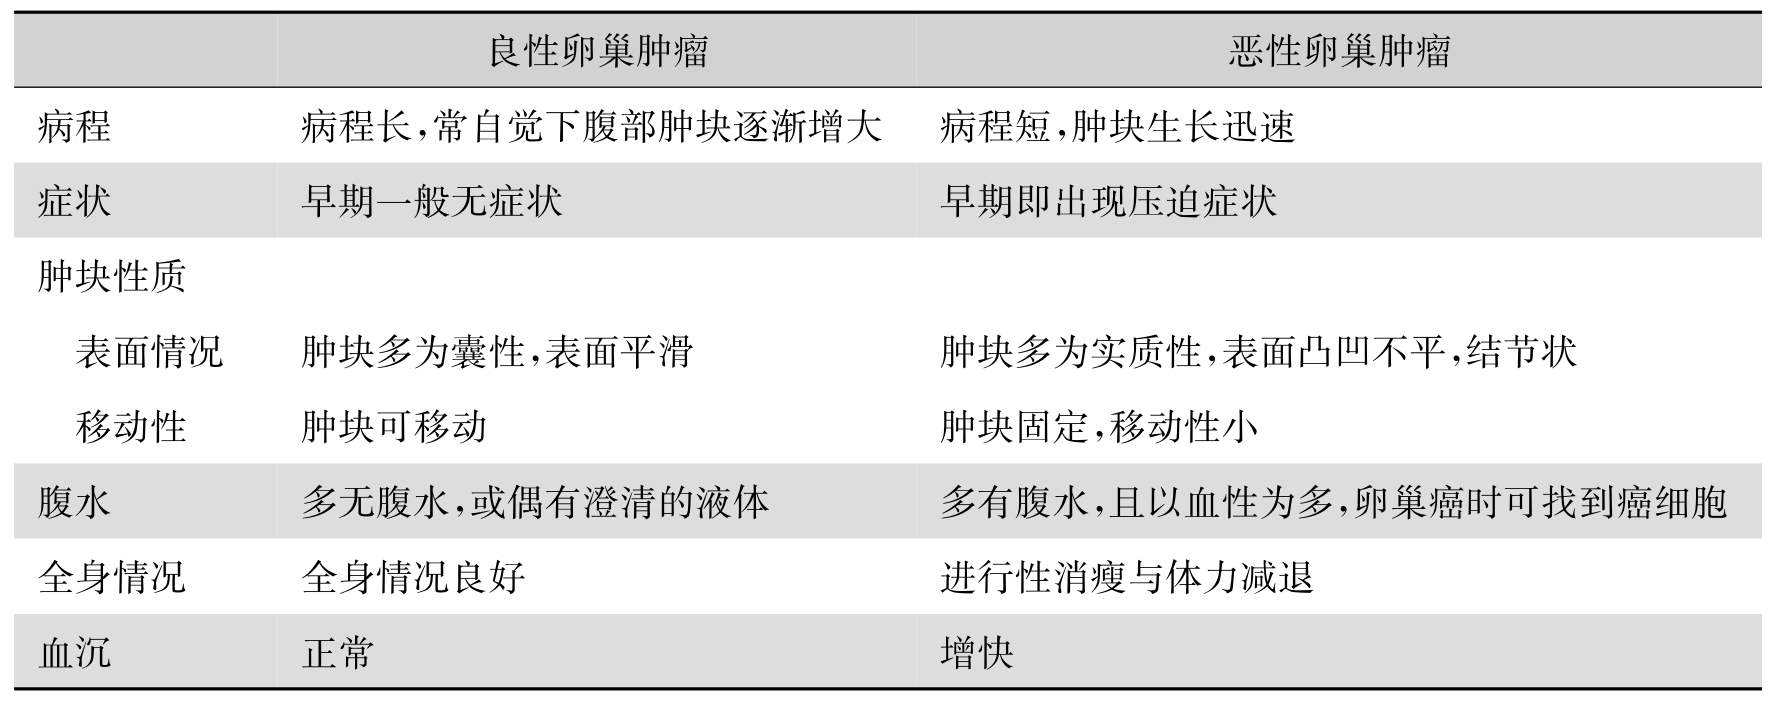
\includegraphics[width=5.90625in,height=2.33333in]{./images/Image00155.jpg}
\end{table}

卵巢克鲁根堡(Krukenberg)瘤

是一种转移性黏液腺癌,绝大多数继发于胃肠道癌,临床上比较少见。患者多以腹部肿块为主诉,常伴有消化系症状。此瘤的临床特点是:①多发生于中年妇女;②有消化系症状,并比盆腔症状先出现;③肿块生长极迅速,多为双侧性,实质性,大小不等,一般如拳头大,外形多保持卵巢原形或类似肾形,表面光滑。

\subsection{十一、双侧性多囊卵巢综合征(Stein-Leventhal综合征)}

病因未明。发生多毛者约占38\%~50\%。多毛一般不显著,常不为患者所注意,仅于体检时才被发现。其主要临床特征为:逐渐进行的月经稀少或闭经,不育,部分患者可伴有肥胖或乳腺发育延迟,卵巢双侧对称性增大,尿17-酮类固醇正常或稍高。B超检查示双侧囊性肿块。腹腔镜检或剖腹探查可明确诊断。特点是:①多发生于中年妇女;②有消化系症状,并比盆腔症状先出现;③肿块生长极迅速,多为双侧性,实质性,大小不等,一般如拳头大,外形多保持卵巢原形或类似肾形,表面光滑。

\subsection{十二、大网膜扭转}

大网膜扭转罕见,本病多发生在右侧腹,可能与右侧网膜体积与活动度较左侧大有关。当存在大网膜疝入疝囊、腹部手术后大网膜游离缘粘连、大网膜包裹炎性病灶、大网膜囊肿、大网膜肿瘤等病理因素时,大网膜易继发扭转,大网膜扭转术前不易诊断,易误诊为急性阑尾炎、腹膜炎等急腹症。CT检查在诊断大网膜疾病有较高的准确性,因此对怀疑大网膜病变者,行螺旋CT检查十分必要。

\protect\hypertarget{text00234.html}{}{}

\section{103 下腹部肿块}

\subsection{一、膀胱肿瘤}

膀胱肿瘤主要的症状是间歇性血尿、尿频与排尿困难。上皮细胞性肿瘤一般向腔内生长或向壁内浸润,腹部触诊触不到肿块,但少数发生于膀胱顶部肿瘤,可在耻骨联合之上触及质硬实的肿块。脐尿管癌好发于中老年人,发病率较低,占膀胱肿瘤的0.55\%~1.20\%。该病常发生于膀胱顶部前壁,肿瘤集中于膀胱壁肌层,可浸润至膀胱壁深层、脐、前腹壁,患者可因腹壁下肿块或脐部有血性溢液就诊,最终诊断依赖病理。非上皮细胞性肿瘤(如肌瘤、纤维瘤、肉瘤等),以耻骨上肿块、排尿困难为主,血尿较少见。膀胱镜检查或膀胱造影对本病的诊断有重要价值,B超可了解肿瘤浸润深度及范围(参见第119.1.4节)。。

\subsection{二、膀胱憩室}

膀胱憩室临床上少见,男多于女,症状多出现在40~60岁。可为先天性,但多继发于尿路梗阻。巨大憩室可于耻骨上部触及肿块。本病一般无症状,部分患者有“两段排尿”现象。膀胱造影或膀胱镜检查可确诊。

\subsection{三、子宫肿瘤}

\subsubsection{(一)子宫肌瘤}

子宫肌瘤是女性生殖器中常见的良性肿瘤,多发生于30~50岁。

一个比较大的肌瘤,下腹部肿块常是患者的主诉之一。其他主要临床症状是月经失常、压迫症状(如盆腔部沉坠感、尿频或尿潴留、便秘、下肢水肿等)、痛经、白带增多等。肿瘤质韧实,表面光滑,位于耻骨上部深处,可向前后及两侧移动,但上下移动度较小;如肿瘤增大,仰卧位也可触及肿瘤上缘的轮廓。此瘤一般根据患者年龄、不育史,以及上述主要的症状与体征,妇科检查发现子宫呈不规则增大、质硬,或触到子宫腔内肿物的下缘便可作出诊断。较大的、呈囊性变的子宫肌瘤常易与卵巢囊肿相混淆;后者无月经过多与痛经,妇科检查可扪到子宫体,肿块位于子宫体旁,与此病不同。在鉴别困难的病例,如患者血压不高,可肌注垂体后叶素5~10U,注射后作腹部触诊,如发现肿块变硬,则有利于子宫肌瘤的诊断。B超对诊断有很大帮助。

\subsubsection{(二)子宫肉瘤}

子宫肉瘤是罕见的恶性肿瘤,大多发生于40岁以上的妇女。子宫肉瘤往往使子宫迅速增大(尤其是在经绝期后的妇女),同时常伴有大量不规则的阴道出血。多数患者有下腹痛。如肉瘤发生溃烂,则有恶臭液体自阴道排出。子宫肉瘤的诊断主要依靠从子宫内刮出肿瘤组织,或手术切除后作病理活检。

\subsubsection{(三)子宫体癌}

子宫体癌多发生于50~60岁的妇女,发现子宫体癌前,往往有功能性子宫出血的存在。当癌弥漫至邻近组织时,有时可在耻骨上部深处触及形状不规则、质坚硬、呈结节状的肿块。宫腔刮出物病理活体组织检查是诊断子宫体癌的可靠方法。B超、CT检查可协助诊断。

\protect\hypertarget{text00235.html}{}{}

\section{104 左下腹部肿块}

\subsection{一、溃疡性结肠炎}

本病主要累及直肠和远端结肠,可向近端发展,以至累及整个结肠,主要症状是腹痛、腹泻、里急后重、黏液脓血便,极少数患者表现为便秘。溃疡性结肠炎的部分病例可在左下腹部触及香肠形肿块,均为挛缩或增厚的结肠。诊断主要依靠结肠镜和病理检查和X线钡灌肠。本病应与结肠癌、结肠克罗恩病等相鉴别。(参见第76.1.2节)。

\subsection{二、乙状结肠癌、直肠癌}

乙状结肠癌逐渐生长,或向邻近组织浸润,可在左下腹触及质硬、不移动的肿块,常表现为便秘、腹泻、大便变细、血便,可伴有低位肠梗阻征象。诊断主要依靠结肠镜检查和X线钡灌肠。直肠癌位于盆腔,腹部触诊不易触及包块,但肛门指检可有阳性发现。主要的临床症状是便血(参见第69.2节)。

\subsection{三、直肠、乙状结肠血吸虫性肉芽肿}

血吸虫病往往侵及直肠、乙状结肠,也可累及盲肠。由于虫卵沉着于肠壁,形成肉芽组织,肠壁增厚,触诊时可触及增厚、变硬的肠管。患者曾有疫水接触史。临床表现主要是腹泻、便血与肝脾大。此病的确诊须靠粪便虫卵孵化法或直肠黏膜活检。较晚期病例孵化法阳性率不高,可在结肠镜窥视下,从直肠黏膜的颗粒样变或黄色小结节处,采取活体组织;或在直肠与乙状结肠交界处及直肠壶腹皱襞之间(约离肛门10~15cm处)的背侧(12点)采取活体组织,虫卵阳性率较高。术后局部涂布次硝酸铋或次碳酸铋粉剂可防止出血,并可避免患者术后下腹疼痛。

\subsection{四、乙状结肠阿米巴性肉芽肿}

乙状结肠及降结肠阿米巴性肉芽肿可在局部形成可触及的肿块。常见的症状是局限性腰痛、体重减轻与肠梗阻。结肠阿米巴性肉芽肿可在晚期出现肠梗阻征象。本病的诊断主要依据:①大便中检出溶组织阿米巴;②钡剂灌肠发现病变肠段狭窄有锯齿状阴影,钡剂通过障碍;③结肠镜检查可见肿块呈葡萄状突入肠腔:附近常有散在性肉芽组织或溃疡存在。此病需与结肠癌鉴别。下列临床表现有助于两者的区别:①患者有痢疾既往史;②阿米巴性肉芽肿常为多发性,而癌则多为单发性;③大便可找到溶组织阿米巴;④阿米巴补体结合试验阳性;⑤经抗阿米巴治疗临床症状迅速好转或消失,肿块显著缩小或消失。

\subsection{五、左侧卵巢肿瘤(参见第102节)}

\subsection{六、乙状结肠憩室炎}

好发于老年男性,多有长期便秘史,急性发作时的表现可酷似左侧阑尾炎,反复发作慢性病例可因多次发生憩室嵌塞性炎症,引起憩室壁炎性增生、肠痉挛性水肿或局部脓肿形成,在左下腹可触及腊肠性肿块,固定而有压痛。诊断主要依靠钡剂灌肠检查,可见肠段呈管状狭窄、充盈缺损及憩室影,肠镜检查可见肠腔狭窄、黏膜炎症,有时可见憩室。但急性期禁忌作肠镜检查,以免引起肠穿孔。

\subsection{七、缺血性结肠炎}

好发于中老年人,90\%发生于60岁以上老年人。典型症状为腹痛、腹泻及血便。可分为非坏疽型和坏疽型,非坏疽型以腹泻为主要临床表现;坏疽型表现为腹痛、便血,可并发肠坏死及肠穿孔。由于供应结肠的动脉发生阻塞导致局部肠壁缺血引起,发病部位左半结肠占80\%,尤其坏疽型多见于结肠脾区和乙状结肠。国内一组报告16例,年龄72~98岁,平均75岁,病程6~32天,多合并高血压、糖尿病、心脑血管疾病及便秘。主要表现腹部肿块,均于腹部左侧触及边界不清的压痛性肿块,其中伴腹痛14例、腹泻7例、便血5例、发热9例。结肠镜示:结肠脾区或乙状结肠黏膜水肿、糜烂呈暗红色,部分有纵行溃疡,黏膜呈结节状,伴有肠管外压性改变,但病变边缘与正常黏膜界限清楚。CT发现左侧腹部肿块呈囊实性或实性,与周围组织界限不清。超声或CT引导下穿刺出脓液或炎性组织支持本病诊断。

\protect\hypertarget{text00236.html}{}{}

\section{105 广泛性与不定位性腹部肿块}

\subsection{一、结核性腹膜炎}

下列两种类型的结核性腹膜炎可形成腹部肿块:

\subsubsection{(一)干酪型结核性腹膜炎}

此型患者以成年人为多,常伴有不规则的发热与其他结核性全身症状。腹部触诊可发现大小不等、界限不清楚、有轻压痛的肿块,叩诊可发现不规则的鼓音区与浊音区,此浊音区的位置常固定。B超提示腹块的存在。此型易被误诊为腹部恶性淋巴瘤或腹膜癌病,但此病多见于30岁以下,大多数有腹膜外结核病灶存在,抗结核治疗疗效佳。腹腔镜检查对诊断帮助颇大。

\subsubsection{(二)粘连型结核性腹膜炎}

此型病例也以成年人为多,经过缓慢,常有顽固性便秘,常因肠绞痛而就诊。体检全身情况一般良好,腹部视诊可见肠蠕动波,触诊有时可发现规则的、境界不清楚的肿块,但无压痛。X线钡餐或(及)腹腔镜检查可证明腹膜粘连。但腹腔镜检查对粘连明显者属禁忌,以防止肠穿孔。偶尔患者因未明原因的急性机械性肠梗阻而住院,经剖腹探查而确诊。

结核性腹膜炎(除已痊愈的粘连型之外)应及早进行抗结核治疗。对高度怀疑本病的病例,也应作抗结核诊断性治疗,既可帮助诊断,又可及时治疗。经诊断性治疗而疗效不佳的病例,手术探查可明确诊断。

\subsection{二、腹型肺吸虫病}

肺吸虫病也可引起广泛性腹膜炎,而产生腹痛、腹泻、腹部压痛与腹块等症状,与结核性腹膜炎相似,但此病是一种地方性寄生虫病,有相应的流行病学史提示诊断(参见第13节)。

\subsection{三、腹部包虫囊肿}

包虫囊肿是人体感染狗绦虫的囊蚴所致的寄生虫病,多见于畜牧地区。患者以20~40岁为多,但在流行病区儿童罹患者也不少见。此病经过缓慢,早期多无自觉症状。腹腔内的包虫囊肿腹部触诊是主要的诊断方法。肿块呈球形,表面光滑而硬韧,以指压之可出现凹陷,并有富于弹性的囊样感,在少数病例可试出震颤感(所谓包虫囊震颤)。早期肿块移动度一般比较大。

女性生殖系统包虫病(棘球蚴病)可发生于卵巢、输卵管、子宫阔韧带和阴道后穹隆等处,下腹部肿块是首先出现的体征,触之呈囊样感,或有波动感。女性的下腹部包虫囊肿须与卵巢囊肿鉴别;位于腰腹部者须与肾囊肿相区别;位于右上腹者须与胆囊积水及肝内非寄生虫性囊肿鉴别。囊肿继续增大,可使全腹膨隆超过足月妊娠的腹围,并引起腹腔器官受压的症状。囊肿突然破裂时可引起过敏性休克。

在疾病过程中常在腹部其他部位发生与原肿块性质相同的新肿块而呈多发性,此与其他原因的囊肿不同,有鉴别诊断意义。B超和CT检查可帮助诊断,包虫皮内试验阳性可帮助确诊。

\subsection{附:包虫囊震颤检查法}

检查者以左手中间三指按压囊肿部位,中指紧压,旁边两指轻轻加压;然后右手中指反复重叩左手中指,每叩之后,叩指应在被叩的左手中指上停留片刻,此时旁边两指即有叩后震颤的感觉。这种感觉和低音级音叉的震动很相似,但不是特征性,在卵巢囊肿时也可出现。

\subsubsection{四、腹膜转移癌}

腹膜转移癌多起源于胃、小肠、肝、胰、结肠、直肠等消化系癌以及卵巢癌、前列腺癌。腹部检查如触及大小不等、形状不规则、质硬实的肿块,可在B超引导下穿刺取标本送病理检查。有弥漫性播散时常产生大量腹水,致肿块难以触及,须放腹水后方能触及,如不能触及包块,可行腹水沉淀找肿瘤细胞,甚至腹腔镜检查。患者常伴有贫血、消瘦与血性腹水。

\subsubsection{五、肠套叠}

肠套叠是婴幼儿中最多见的急性肠梗阻疾病,约90\%患儿在2岁以下。成人和年长儿童,症状较不典型,便血的现象较少。

腹部肿块出现的部位,随肠套叠的类型与病程进展程度而不同。小肠套叠的肿块多在脐周,较小,移动性较大。回盲部套叠肿块通常在右下腹,呈香蕉形,质较硬,表面平滑,稍可移动。肿块在腹痛发作时变硬,而在间歇期质较软。阵痛每发作一次,肿块就加大范围而推进一步。肠套叠的肿块应在无痛的间歇期间触诊;柔软而能推动的肿块,是其特征。在腹绞痛发作时,用听诊器可听到增强的肠鸣音。诊断有怀疑时,用水合氯醛溶液灌肠,使患者腹肌松弛,可增加触诊的阳性率。钡剂灌肠检查有确诊价值,但对小肠套叠无帮助,可行腹部CT检查。

\subsubsection{六、肠梗阻}

肠梗阻可由肠腔内因素、肠壁因素和肠外因素引起。临床上以腹痛、腹胀、呕吐、腹块和肛门停止排气排便为主要表现,症状随梗阻的程度、梗阻部位的高低,以及梗阻原因等的不同而有所区别。不完全性肠梗阻仍有肛门排气排便,完全性肠梗阻在梗阻远端的肠内容物未排净之前,患者也可继续排气排便。高位肠梗阻者呕吐频繁,腹胀不明显,而低位肠梗阻则呕吐出现较晚,且不如高位肠梗阻者频繁,腹胀比较明显。若梗阻在结肠,可仅有腹胀而无呕吐。机械性肠梗阻因肠蠕动增加,常有阵发性腹痛伴肠鸣。持续性腹痛伴阵发性加剧是早期绞窄性肠梗阻的特点,病情继续发展可出现剧烈的持续性腹痛,甚至休克。X线检查显示小肠有多个气液平面,结肠肠腔明显扩张,并可见结肠袋,多为结肠梗阻。

腹茧症为一罕见的腹膜病变,即腹腔部分或全部脏器被一层膜样物质包裹,形似蚕茧。好发于青少年女性,尤其是有月经不调及不孕史者,常表现腹痛、腹胀、腹部包块、呕吐等急性或慢性肠梗阻症状。对反复出现急性或慢性肠梗阻症状,而无其他原因解释或合并腹部包块者应考虑腹茧症可能,术前放射学检查及腹腔镜检查对本病诊断很有价值。确诊依靠术中所见及术后纤维膜病理学检查。腹茧症还需与腹膜包裹症鉴别,腹膜包裹症患者小肠被包绕在一层相对正常的腹膜中,其内壁与小肠肠管并无粘连,肠梗阻的发生率低。

\subsubsection{七、肠扭转}

肠扭转临床表现为急性机械性肠梗阻,占肠梗阻的10\%~20\%,以小肠最多见,占肠扭转的80\%,其次为乙状结肠与盲肠。饱餐后剧烈或过度用力常为诱因。肠发生扭转时,患者出现阵发性剧烈腹痛、呕吐与腹胀。结肠扭转时呕吐出现较晚,而腹胀最为显著,腹部常可触及有弹性、压痛的肿块,叩诊呈鼓音。X线检查见肠梗阻征象及双袢肠曲,肠管呈倒“U”字形排列,CT显示肠系膜上动脉呈“漩涡征”、血管变细或突然中断。钡灌肠钡剂通过受阻及出现“鸟嘴”征。

\subsubsection{八、腹膜假黏液瘤(pseudemyxoma peritonei,PMP)}

是一种少见的临床综合征,特点为腹腔内充满黏液样液体和胶冻状肿物。国内一组报告33例,男性11例,女性22例,平均年龄50岁,发病至确诊中位间期为12个月,误诊率为84.8\%。主要表现为腹胀、腹部包块、腹痛不适、腹围增大等,病灶主要分布于回盲部、腹膜、网膜、卵巢附件、膈下、直肠前凹等。腹部B超、CT可发现具有回声的流动性差的腹水征、腹膜及网膜饼样增厚、肝脾表面扇形压迹等,腹水难以抽出。确诊靠B超引导下穿刺活检、腹腔镜及手术探查。33例中良性22例,中间性7例,恶性4例。

\subsubsection{九、腹部Castleman病}

Castleman病又称血管滤泡性淋巴组织增生或巨大淋巴结增生,是一种原因不明的慢性淋巴组织增生性疾病,常为不明原因的淋巴结肿大,以纵隔、颈部、腋下好发,腹腔及腹膜后少见。国内一组腹部Castleman病17例报告,男6例,女11例,年龄11~58岁,平均36.8岁。11例无任何症状,因腹部B超发现,2例可扪及腹部包块,2例表现为口腔溃疡、皮疹,1例表现为上腹隐痛、恶心、呕吐,1例表现为水肿、气短。病灶位于腹膜后12例,肠系膜3例,肾上腺周围2例,直径为1.5~9.0cm,其中13例为单发,3例为腹膜后多发,1例为大网膜和腹膜后多发。4例术前经CT诊断为Castleman病,其余13例未明确诊断,确诊依赖术后的病理检查。

\subsubsection{十、腹膜恶性间皮瘤}

腹膜恶性间皮瘤是原发于腹腔浆膜的恶性肿瘤。临床表现无特异性,常为腹胀、腹痛、腹部包块、腹水增长较快,为血性或浆液性。B超、CT检查发现腹水、腹腔包块、腹膜不规则增厚。腹水细胞学检查、腹腔镜检查、活检病理可明确诊断,必要时剖腹探查。

\subsubsection{十一、炎症性肌纤维母细胞瘤(inflammatory myofibroblastic tumor,IMT)}

IMT是主要发生于软组织和内脏的少见的间叶性肿瘤,目前已将IMT归入中间性(偶有转移性)的肌纤维母细胞(成纤维细胞)肿瘤中。该病常见发生部位在肺部,人体多个器官均可发生。肺外IMT的好发部位是大网膜、肠系膜、腹膜后,多发生于儿童及年轻人,临床表现为发病部位出现肿块,及随发病部位而异的症状,如腹痛、肠梗阻、腹水等,诊断依赖病理检查。

\protect\hypertarget{text00237.html}{}{}

\section{参考文献}

1.北京市肿瘤防治研究所,等.胃肉瘤36例的临床和胃镜表现.中华内科杂志,1978,17:361

2.吴新彦,等.胃恶性淋巴瘤的临床X线诊断.中华医学杂志,1977,57:155

3.柳凤轩.胃肠道恶性平滑肌肿瘤的诊断与预后的关系.中华内科杂志,1985,24:149

4.陆星华.原发性小肠肿瘤97例分析.中华内科杂志,1986,25:31

5.周惠邦.胃扭转7例报告.北京医学,1985,7:82

6.田文彪,等.胃扭转17例报告.中华放射学杂志,1979,13:168

7.郑显理,等.胰腺囊肿的诊断与外科治疗.中华外科杂志,1979,17(4):238

8.陈海琼,等.胰腺囊腺瘤四例报告.中华内科杂志,1965,13:837

9.朱人瑞.胰腺囊肿的诊断和治疗.上海医学,1981,4:327

10.王一川,等.大网膜肿瘤与囊肿的诊断与治疗.中华外科杂志,1979,17:136

11.方大维,等.腹主动脉瘤的诊断和治疗(附10例分析).新医学,1980,11(1):13

12.龙子雯,等.原发性腹膜后肿瘤200例诊治分析.中国实用外科杂志,2013,73(2):127

13.李运康.巨大肾积水25例报告.中华外科杂志,1982,20:459

14.韩莘野.肾区肿块的X线诊断与鉴别诊断.上海医学,1979,2(5):42

15.陈宜和.巨大肾积水.中华外科杂志,1964,12(11):1069

16.高洪深.蹄铁形肾三例报告.中华外科杂志,1964,12(4):358

17.黄席珍.化学感觉器瘤的诊断和治疗.中华内科杂志,1978,17:193

18.唐振铎,等.回盲部病变的鉴别诊断.中华内科杂志,1965,13:411

19.胡秀媛.麦格氏综合征二例报告.中华妇产科杂志,1978,13:128

20.顾人勋,等.14例卵巢克鲁根堡氏瘤临床病理分析.中华妇产科杂志,1964,10:211

21.罗惠文.卵巢含睾丸细胞瘤一例报告.中华妇产科杂志,1963,9:236

22.陈壁华.卵巢肾上腺皮质瘤一例.中华妇产科杂志,1979,14:18

23.杜心.双侧卵巢多囊综合征.中华妇产科杂志,1963,9:145

24.陆湘云.多囊卵巢综合征.上海医学,1984,7:172

25.苏州医学院第一附属医院.血吸虫病性大肠肉芽肿的临床与病理研究.中华医学杂志,1977,57:623

26.梁圣保.肠阿米巴肉芽肿附五例报告.中华内科杂志,1964,12:561

27.侯家珠.女性生殖系统包虫病(综述).中华妇产科杂志,1981,16(2):115

28.顾倬云,张国华.假性胰腺囊肿20例临床分析.中华消化杂志,1995,15(5):238

29.陈伟光,等.小肠平滑肌肉瘤26例误诊分析.中华消化杂志,1997,17(2):76

30.王为服,等.肾上腺囊肿的诊断及治疗.中华外科杂志,1998,36(2):127

31.李澍,等.原发性腹膜后肿瘤.中华外科杂志,1997,35(11):648

32.江玮,等.肾上腺皮质腺癌20例报告.中华外科杂志,1995,33(10):621

33.孔垂泽,等.无功能肾上腺肿瘤29例临床分析.中华外科杂志,1995,33(9):557

34.袁祖荣,等.对原发性小肠肿瘤的几个问题的探讨------附86例临床分析.中华消化杂志,1991,11(5):264

35.陈祖望,等.CT在腹主动脉瘤的诊断价值.中华心血管病杂志,1992,20(6):361

36.阿斯甫江,阿斯亚.肾包虫病的诊断及治疗(附28例报告).中华泌尿外科杂志,2000,21(10):602

37.徐明谦,等.肝囊性包虫病的影像学诊断与分型.中华医学杂志,2002,82(3):176

38.李坤鹏,等.特发性腹膜后纤维化61例临床特征并文献分析.中华内科杂志,2009,48(11):912

39.何晓东,等.先天性胆总管囊肿56例诊治经验.中华外科杂志,2000,38(3):235

40.郑家驹,等.克罗恩病的临床多样症状.中华消化杂志,2002,22(4):226

41.王爱英,林三仁.小肠双重造影1182例总结.中华消化杂志,2005,25(5):262

42.钟捷,等.双气囊小肠镜与胶囊内镜诊断小肠出血病因比较.中华消化杂志,2004,24(12):741

43.程邦君,等.腹茧症的临床特点及诊疗进展.中华消化杂志,2012,32(1):68

44.沈旺,等.胃肠道及胃肠道外间质瘤216例临床病理学特点分析.中国实用外科杂志,2011,31(8):693

45.井方方,等.国内胰腺实性假乳头状瘤1180例临床荟萃分析.中华胰腺病杂志,2013,13(2):98

46.李乐,等.肠系膜囊肿的诊断与治疗.中华消化外科杂志,2013,12(6):469

47.余晨,肖香佐.多排螺旋CT小肠造影在评估小肠克罗恩病中的应用.世界华人消化杂志,2013,21(3):233

48.王柏棻,钟捷.影像学诊断在炎症性肠病中的应用.国际消化病杂志,2013,33(1):3

49.孟欣颖,周长宏.胶囊结肠镜的临床应用.胃肠病学,2013,18(1):55

50.刘允怡,等.自身免疫性胰腺炎与胰腺癌的鉴别诊断.中华消化外科杂志,2013,12(2):96

51.方薛泉,等.腹部Castleman病的临床诊断和治疗.中华消化外科杂志,2010,9(4):273

52.李晓伟,等.盆腔腹膜后肿瘤16例临床分析.中华医学杂志,2013,93(17):1327

53.王宁,等.回盲部炎性包块241例临床特征分析.中华消化杂志,2013,33(2):97

54.彭伟彬,等.脐尿管癌的临床诊断及治疗.国际外科学杂志,2013,40(1):33

55.吴朝阳,等.自身免疫性胰腺炎误诊为胰腺癌原因辨析.临床误诊误治,2013,26(5):26

56.张小文,王炳煌.大网膜扭转.中国医师进修杂志,2008,31(5):8

57.郭宏荣,等.以腹部肿块为主要表现的老年缺血性结肠炎16例.人民军医,2013,56(2):209

58.宋志强,等.腹膜假黏液瘤的临床病理特征和预后分析.中华内科杂志,2005,44(12):894

59.宋保平,岳志红.间断腹痛、腹部肿块1年余.新医学,2008,39(10):631

\protect\hypertarget{text00238.html}{}{}

